\documentclass[a4paper,11pt]{report}
\usepackage[T1]{fontenc}
\usepackage[utf8]{inputenc} 
\usepackage[english]{babel} 
\usepackage{url}
\usepackage{graphicx}
\usepackage{lipsum}
\usepackage{tocbibind} 
\usepackage{booktabs}
\usepackage{colortbl}
\usepackage[table]{xcolor}
\usepackage[dvisvgm, usenames, dvipsnames]{color}
\setlength{\arrayrulewidth}{0.5mm}
\setlength{\tabcolsep}{18pt}
\renewcommand{\arraystretch}{2.5}
\usepackage{longtable}
\usepackage{array}
\newcolumntype{C}[1]{>{\centering\let\newline\\\arraybackslash\hspace{0pt}}m{#1}}
\usepackage{url}							
\usepackage{hyperref}
\usepackage{enumitem}
\usepackage{float}
\restylefloat{table}
\usepackage{xltabular}
\usepackage{xcolor}
\definecolor{green1}{HTML}{85AB67}
\definecolor{green2}{HTML}{77BC3F}
\usepackage{pdflscape}
\usepackage{pdfpages}
\setcounter{secnumdepth}{3}
\usepackage{wrapfig}
\usepackage{multicol}
\usepackage{graphicx}
\usepackage{listings}
\usepackage{color}
\usepackage{geometry}
\definecolor{lightgray}{rgb}{.9,.9,.9}
\definecolor{darkgray}{rgb}{.4,.4,.4}
\definecolor{purple}{rgb}{0.65, 0.12, 0.82}

\lstdefinelanguage{JavaScript}{
  keywords={typeof, new, true, false, catch, function, return, null, catch, switch, var, if, in, while, do, else, case, break},
  keywordstyle=\color{blue}\bfseries,
  ndkeywords={class, export, boolean, throw, implements, import, this},
  ndkeywordstyle=\color{darkgray}\bfseries,
  identifierstyle=\color{black},
  sensitive=false,
  comment=[l]{//},
  morecomment=[s]{/*}{*/},
  commentstyle=\color{purple}\ttfamily,
  stringstyle=\color{red}\ttfamily,
  morestring=[b]',
  morestring=[b]"
}

\lstset{
   language=JavaScript,
   backgroundcolor=\color{lightgray},
   extendedchars=true,
   basicstyle=\footnotesize\ttfamily,
   showstringspaces=false,
   showspaces=false,
   numbers=left,
   numberstyle=\footnotesize,
   numbersep=9pt,
   tabsize=2,
   breaklines=true,
   showtabs=false,
   captionpos=b
}



\begin{document}

\begin{titlepage}

\newcommand{\HRule}{\rule{\linewidth}{0.1mm}}

\center 


\includegraphics[width=50mm,scale=0.5]{./Images/Logo_Politecnico_Milano.png}\\[0.5cm] 

{\Large Computer Science and Engineering}\\[0.4cm] 
{\large Design and Implementation of Mobile Applications}\\[0.4cm] 
{\large Academic year 2021-2022}\\[0.5cm] 

\HRule \\[1 cm]
{\LARGE \textbf{Design Document}} \\[0.7cm]
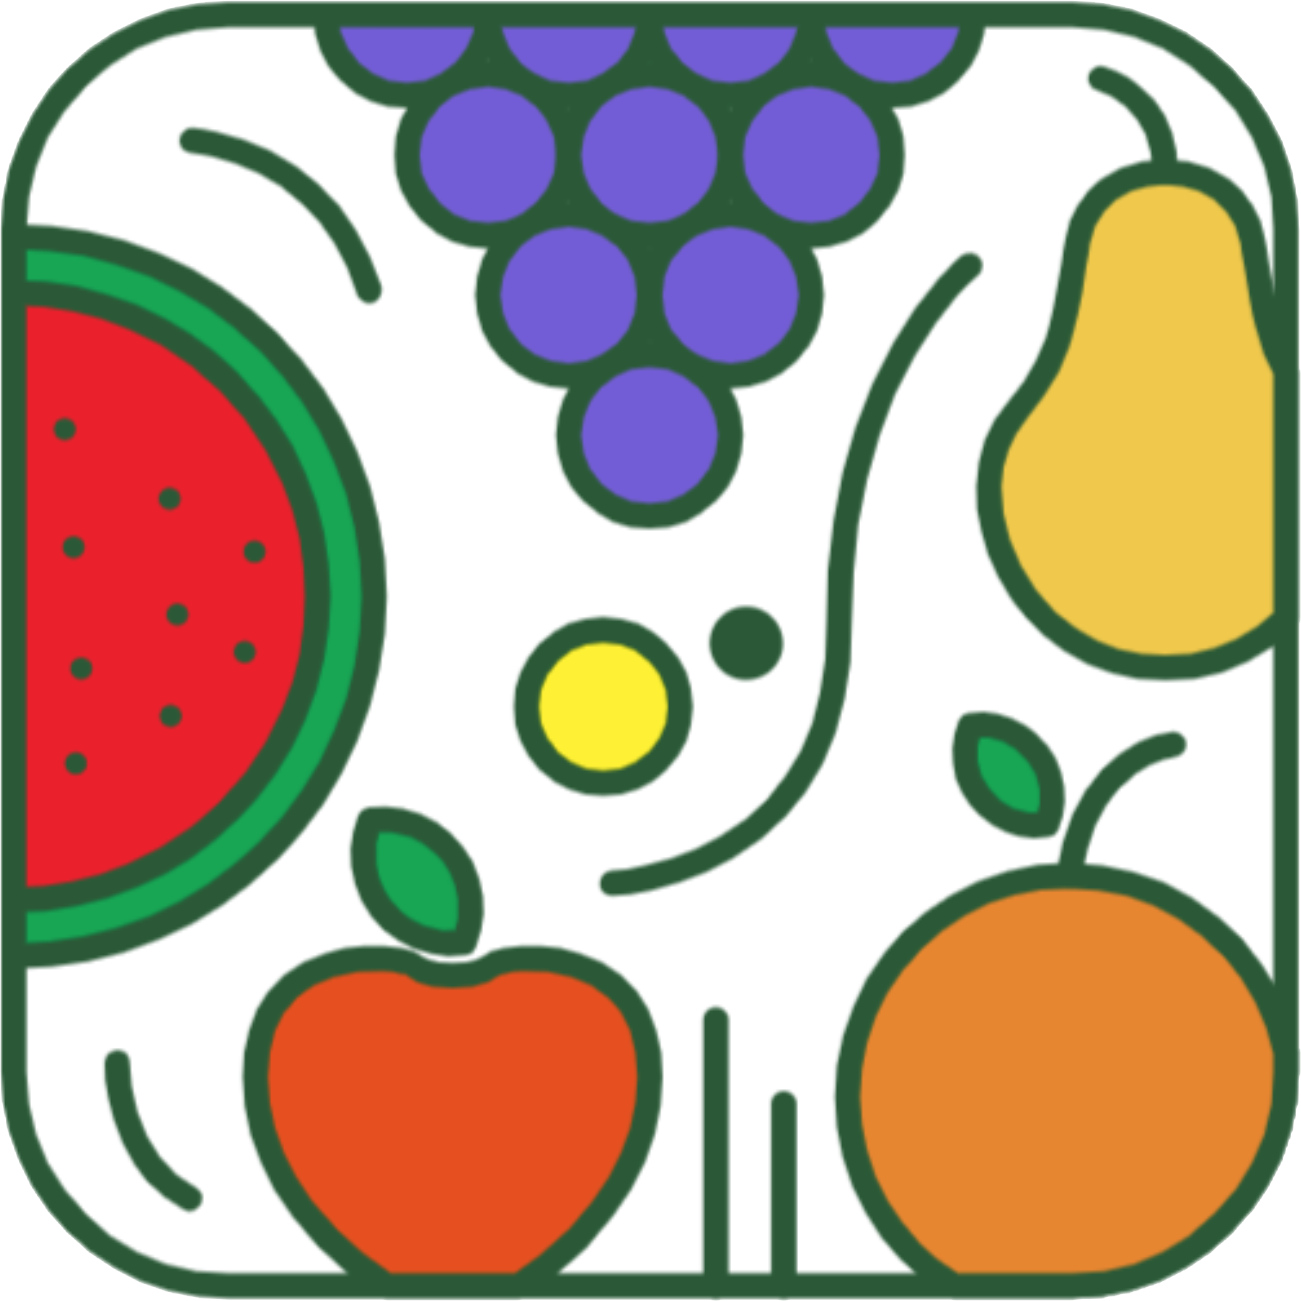
\includegraphics[width=35mm,scale=0.5]{./Images/Logo/expiry_app_logo.png}\\[0.5cm] 
{\LARGE Expire App} \\[0.7cm]
\HRule \\[1cm]
\raggedright

\begin{minipage}{0.55\textwidth}
\begin{flushleft} \large
\emph{Authors:}\\
Arslan \textsc{Ali}\hfill 10807090 \\
Alessandro \textsc{Sorrentino}\hfill 10746269 \\
\end{flushleft}
\end{minipage}\\[0.7 cm]
~

\center

%{\large January -, 2022}\\[0.3 cm]
{\large Version 1.0}\\

\vfill 
\end{titlepage}

\newpage

\addtocontents{toc}{\protect\setcounter{tocdepth}{-1}}
\tableofcontents
\addtocontents{toc}{\protect\setcounter{tocdepth}{3}}
\listoftables
\newpage
\listoffigures
\newpage

\chapter{Introduction}


\section{Purpose}
The goal of DD (Design Document) is to provide a more extensive overview of the architectural decisions, their communication interfaces, made to implement all the functionalities described in the RASD document.
In the last chapter (5) it will also present implementation, integration and test plan.

\subsection{Goals}

Lorem ipsum dolor sit amet, consectetur adipiscing elit. Fusce bibendum est vel tincidunt tristique. Pellentesque congue, nulla et sollicitudin ultrices, tellus urna blandit odio, et malesuada est tellus vitae eros. Sed id ipsum a nibh mattis posuere vel nec risus. Pellentesque vestibulum malesuada sapien, et rhoncus enim blandit a. Etiam lacinia accumsan est. Nullam et turpis eget lectus semper pharetra. Pellentesque finibus dui at elementum viverra. Morbi mattis posuere libero eu feugiat. Fusce nec erat urna. Suspendisse potenti.
\section{Scope}
As stated in the RASD document, the aim of the DREAM software product is to develop and adopt anticipatory governance models for food systems to strengthen data-driven statepolicy. It takes care of the acquisition and management of all data collected in order to support the work of farmers, agronomists and policy makers. The system aims to collect data not only from sensors located throughout the territory, but also from farmers. The analysis of the acquired data aims to improve the production of farmers. Low-performing farmers are identified by policy makers and helped by the best-performing ones. Everything is supervised by agronomists who take care of their own geographical areas of competence.

\section{Definitions, Acronyms, Abbreviations}

In the following section is clarified the meaning of some definitions, acronyms and abbreviations which will be use in the DD, in order to help the general understanding of the document.

\newpage
\subsection{Definitions}
\begin{center}
\setlength\tabcolsep{7pt}
\rowcolors{2}{white}{white!65!green2!50}
\renewcommand{\arraystretch}{2}
\begin{longtable}{|m{3.2cm}|m{8.3cm}|}
\caption{Definitions}\\
\hline
\endfirsthead
\endhead
\hline
\endlastfoot
\textit{The system} & The whole system to be developed \\
\textit{User} & A farmer/agronomist/policy maker who uses the application\\
\textit{Unregistered user} & A farmer/agronomist/policy maker who is not yet registered into the application\\
\textit{Application service} & Functionality offered by the system for certain users \\
\textit{Policy maker} & The user of the application who decides about new policies for Telangana \\
\textit{Farmer} & The user of the application who owns or manages a farm\\
\textit{Address} & The address inserted by the farmer which corresponds to his/her farm's location. It is composed by city, zip code, street and number\\
\textit{Performance} & Indicator of the progress of a farmer's activity up to a certain date. Its value is calculated as numerical score \\
\textit{Score} & Performance rating computed by a function that depends on: type and quantity of harvested product, weather conditions, quantity of water consumed, soil moisture\\
\textit{Well performing farmer} & A farmer who has a score higher than a certain threshold\\
\textit{Bad performing farmer} & A farmer who has a score below a certain threshold\\
\textit{Agronomist} & The user of the application dealing with the management of a certain mandal\\
\textit{Mandal} & A local government area and  administrative division. Telangana is subdivided into districts which are themselves subdivided into mandals\\
\textit{Daily plan} & Application service that allows the agronomist to manage his/her daily work schedule. Specifically, it allows him/her to track and organize visits to farmers\\
\textit{Discussion forum} & Application service which a farmer can use to exchange ideas and opinions about a topic\\
\textit{Post} & Contributions of the participants to the discussion placed one below the other in sequence\\
\textit{Thread} & It is composed of the topic followed by the posts left by the various participants in the discussion\\
\textit{Help request} & Application service which a farmer can use to request for help to the agronomist or/and other well performing farmers\\
\end{longtable}
\end{center}
\subsection{Acronyms}

\begin{center}
\setlength\tabcolsep{7pt}
\rowcolors{2}{white}{white!65!teal!40}
\renewcommand{\arraystretch}{2}
\begin{longtable}{|m{1.5cm}|m{8.6cm}|}
\caption{Acronyms}\\
\hline
\endfirsthead
\endhead
\hline
\endlastfoot
\hline
\textit{DD} & Design Document\\
\textit{DBMS} & Database Management System\\ 
\textit{DB} & Database\\
\textit{UML} & Unified Modelling Language\\
\textit{API} & Application Programming Interface\\
\textit{UI} & User Interface\\
\textit{HTTP} & Hypertext Transfer Protocol\\
\textit{ID} & Identification\\
\textit{JSON} & JavaScript Object Notation\\
\textit{OCR} & Optical Character Recognition\\
\hline
\end{longtable}
\end{center}
\subsection{Abbreviations}

\begin{center}
\setlength\tabcolsep{7pt}
\rowcolors{2}{white}{white!65!green2!50}
\renewcommand{\arraystretch}{2}
\begin{longtable}{|m{1.5cm}|m{8.6cm}|}
\caption{Abbreviations}\\
\hline
\endfirsthead
\endhead
\hline
\endlastfoot
\hline
\textit{G.i} & i-th goal\\
\textit{R.i} & i-th requirement\\
\textit{D.i} & i-th domain assumption\\
\textit{UC.i} & i-th use case\\
\hline
\end{longtable}
\end{center}
\section{Document Structure}

The DD is structured in the following five chapters:
\begin{itemize}
\item \textbf{Chapter 1 -  \textit{Introduction}:} 

\item \textbf{Chapter 2 -  \textit{Overall description}:} 

\item \textbf{Chapter 3 -  \textit{Architectural design}:} 

\item \textbf{Chapter 4 -  \textit{User interface design}:} 

\item \textbf{Chapter 5 -  \textit{Implementation, Integration and Test Plan}:}

\end{itemize}
\chapter{Overall description}

In this chapter are reported the main architectural design choices from a high level point of view. In the following sections are presented the chosen paradigm of the system and its components, followed by the description of how the system will be deployed. Moreover, components’ sequence and interface  diagrams are listed to describe the way components interact to accomplish specific tasks of the application. Eventually, the last two sections provide specifications regarding the selected architectural style and other design choices.

\section{Product perspective}

\textit{Expire App} is a system that provides all the functionalities described in the product functions section. It includes all the subsystems needed to fulfil these software requirements. User can access the service through the application, which should be downloadable and runnable both on iOS and Android devices either phone or tablet. All interfaces must conform to a uniform, intuitive and user-friendly design, that doesn't require the reading of detailed documentation to be used. The mobile application can run on devices that comply with the minimum requirements in terms of memory and screen size, computational power and other relevant parameters specified in the subsection 2.5. Furthermore, the back-end services are all hosted by Google’s Firebase.

\newpage

\section{External services}
In the next subsections, the main external services used in the application will be illustrated and briefly explained.

\subsection{Firebase}
\begin{wrapfigure}{R}{0.3\textwidth}
\vspace{-0.8cm}

\includegraphics[width=0.18\textwidth]{Images/external_serv/firebase.png}
\end{wrapfigure}
Firebase is a Backend-as-a-Service (Baas). It provides a variety of tools and services.It is built on Google’s infrastructure. Firebase is categorized as a NoSQLdatabase program, which stores data in JSON-like documents.
Firebase offers multiple backend services, of which Expire App uses:
\begin{itemize}
    \item Firebase Authentication: is an extensible token-based auth system and provides out-of-the-box integrations with the most common providers such as Google, Facebook, and Twitter, among others.
    \item Firestore Database: cloud-based NoSQL database server that stores and sync data, that supports automatic scaling. It stores data as documents that are logically classified into collections. The Firestore document offers support for multiple file types, numbers, strings, and nested objects.
    \item Cloud Storage: is an object storage service. In Expire App it's used for storing pictures of products
\end{itemize}


\subsection{OpenFoodFacts}
\begin{wrapfigure}{R}{0.3\textwidth}
\vspace{-0.8cm}

\includegraphics[width=0.25\textwidth]{Images/external_serv/openfoodfacts1.png}
\end{wrapfigure}

Open Food Facts is a free, online and crowdsourced database of food products from around the world licensed under the Open Database License (ODBL).
In Expire App it's involved when a user add a product by scanning barcode.
The database contains mostly food products and their details, such as nutritional values.
Those data is also used in the statistics screen, to create charts regarding nutritional values.
\newpage

\subsection{Spoonacular API}
\begin{wrapfigure}{R}{0.3\textwidth}
\vspace{-0.8cm}

\includegraphics[width=0.20\textwidth]{Images/external_serv/spoonacular.png}
\end{wrapfigure}
Spoonacular is a recipe search engine and social cooking platform. In Expire App  this service is used whenever the user tap on the recipe section.
This API provides a list of recipes based on the ingredients that the user has already saved, it's also possible to get detailed information about a recipe by tapping on it.\newline

\subsection{Google Cloud Vision API}
\begin{wrapfigure}{R}{0.3\textwidth}
\vspace{-0.8cm}

\includegraphics[width=0.20\textwidth]{Images/external_serv/vision_api.png}
\end{wrapfigure}
This service is a OCR offered by Google.
It permits the conversion of handwritten/printed texts into machine-encoded text, in Expire App it used when a user adds a new product manually, and instead of writing the list of ingredients manually, he/she can take a picture of the label, and the service will translate it into text.

\subsection{Authentication}
Firebase Authentication provides backend services. It supports authentication using passwords, phone numbers, popular federated identity providers like Google, Facebook and Twitter, and more.

\subsubsection{Google authentication}
\begin{wrapfigure}{R}{0.3\textwidth}
\vspace{-0.8cm}

\includegraphics[width=0.20\textwidth]{Images/external_serv/g.png}
\end{wrapfigure}
Authentication into Expire App using a Google account, 3rd party library is required to trigger the authentication flow, called \textit{google\textunderscore sign\textunderscore in}.
\newpage

\subsubsection{Facebook authentication}
\begin{wrapfigure}{R}{0.3\textwidth}
\vspace*{-0.8cm}

\includegraphics[width=0.13\textwidth]{Images/external_serv/f.png}
\end{wrapfigure}
Like Google authentication, also Facebook authentication required a 3rd party library, called \textit{flutter\textunderscore facebook \textunderscore auth} and some manual adjustment with native settings for android and iOS. To use Facebook authentication it's needed a Facebook account and access the Facebook Developer Platform. Facebook provides an authentication token that can be used via OAuth for authorization and log in into Firebase.\newline

\subsubsection{Apple authentication}
\begin{wrapfigure}{R}{0.3\textwidth}
\vspace{-0.8cm}
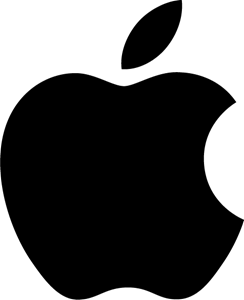
\includegraphics[width=0.13\textwidth]{Images/external_serv/a.png}
\end{wrapfigure}
Authentication into Expire App using a Apple account (possible only for iOS and iPadOS users).\newline

\subsection{Scandit}
\begin{wrapfigure}{R}{0.3\textwidth}
\vspace{-0.8cm}

\includegraphics[width=0.20\textwidth]{Images/external_serv/scandit.png}
\end{wrapfigure}
Scandit is a platform for mobile computer vision and augmented reality, it offers a variety of products, in Expire App we used the barcode scanner for reading:
\begin{itemize}
    \item barcode: when a user want to insert a new product to the list
    \item qrcode: when a user want to join a family group
\end{itemize}
\newpage
\section{Assumptions and dependencies}
\begin{itemize}
    \item [\textit{D.1}] To authenticate the user needs an internet connection
    \item [\textit{D.2}] User must have access to a camera
    \item [\textit{D.3}] All the family members live together and trust each other
   
\end{itemize}


\def\fillandplacepagenumber{%
 \par\pagestyle{empty}%
\vbox to 0pt{\vss}\vfill
\vbox to 0pt{\baselineskip0pt
   \hbox to\linewidth{\hss}%
   \setlength{\footskip}{70pt}
   \baselineskip\footskip
   \hbox to\linewidth{%
     \hfil\thepage\hfil}\vss}}




\section{Functional requirements}
This section shows the physical distribution of the system, that is, the environment in which the system runs. Specifically, \textit{Figure 2.4} shows the structure of the hardware components that execute the software.

Firewalls are inserted to ensure security between the different zones and load balancers are designed to distribute the workload.\\

As previously mentioned, the system is divided into 4 Tier, the components of which are described below:
\begin{itemize}
    \item \textbf{Client Tier}: it consists of the client programs used to exploit system services and the devices on which these programs are installed.
    \begin{itemize}
        \item \textbf{Smartphone}: users access the DREAM system and use the related services through a mobile application from a smartphone.
        \item \textbf{Personal Computer}: users access the DREAM system and use the related services through the Web browser from a personal computer.
    \end{itemize}
    \item \textbf{Web Tier}: it consists of components that handle the interaction between client tier and the business tier.  It contains the Web Server.
    \begin{itemize}
        \item \textbf{Web Server}: it provides content to the Web using the HTTP(S) protocol. It mainly works to serve the requested web pages continuously and without interruption. As long as the Web Server is up and running, the corresponding web pages and sites will be available to users on the network.
    \end{itemize}
    \item \textbf{Business Tier}: it processes all dynamic content and the interactions between the Client/Web Tier and the Data tier. It contains the Application Server.
    \begin{itemize}
        \item \textbf{Application Server}: it hosts and exposes business logic and processes. It provides the infrastructure and logical capabilities to support, develop and run applications in a distributed context. The Application Server communicates directly with the Mobile Application through HTTPS protocol, in order to create a lightweight API to request only the necessary data. The Application Server will receive this call, make the call to the external service, filter it, and return only what the application has requested.  This will reduce the amount of data transiting over mobile Internet and thus increase application performance.
    \end{itemize}
    \item \textbf{Data Tier}: it runs the DBMS and holds all of the sensitive application data. It contains database servers.
    \begin{itemize}
        \item \textbf{Database Server}: it allows access to one or more Database Systems and is an essential support for Web Servers in managing the delivery and storage of data. It communicates with the Application Server via the standard TCP/IP protocol and provides access to the physical database which is in charge of storing all persistent data of users who use DREAM.
    \end{itemize}
\end{itemize}\\


\textbf{Firewalls} are also included in the system architecture to delimit safe areas within the system. 
Specifically, there are firewalls between the Internet accessed by the customer to use the application and the Web Server and between the latter and the Application Server in order to create a demilitarized zone (DMZ). The purpose of the DMZ is to add an additional level of security to an internal network, where a node belonging to an external network can only access the services made available, without putting at risk and compromising the security of the entire network.
In order to ensure secure access to the database and to delimit the internal network (IN), a firewall is placed between the Application Server and the Database Server.\\


In order to distribute the load of the requests to the DREAM website among several servers, \textbf{load balancers} are introduced for the Web Server. In this way, the reliability and scalability of the entire architecture increases because requests will be shared equally among the different servers. If one of the servers is unable to respond to the request, the user can still use the service based on one of the active servers.
Similarly, the Web Server may need to query the database to generate responses. Web Servers send database queries to the load balancer which balances the inbound database workload on the database servers.



\def\fillandplacepagenumber{%
 \par\pagestyle{empty}%
\vbox to 0pt{\vss}\vfill
\vbox to 0pt{\baselineskip0pt
   \hbox to\linewidth{\hss}%
   \setlength{\footskip}{70pt}
   \baselineskip\footskip
   \hbox to\linewidth{%
     \hfil\thepage\hfil}\vss}}






\section{User characteristics}
We consider users every person who downloaded the application on his/her device (Android, iOS or iPadOS).
The actors of the applications are the following:
\begin{itemize}
    \item \textit {Unregistered user}: a person who has not registered and is allowed to use the application with limited functionalities.
    \item \textit {User}: a person who is already registered into the application.
\end{itemize}




\def\fillandplacepagenumber{%
 \par\pagestyle{empty}%
\vbox to 0pt{\vss}\vfill
\vbox to 0pt{\baselineskip0pt
   \hbox to\linewidth{\hss}%
   \setlength{\footskip}{70pt}
   \baselineskip\footskip
   \hbox to\linewidth{%
     \hfil\thepage\hfil}\vss}}









\section{Constraints}

\subsection{Regulatory policies}
\subsection{Hardware constraints}
\subsection{Availability}
It refers to the system’s ability to be available for use, especially after a failure has occurred. The fault must be recognized and then the system must
respond in some way. The system should be available for 99.97\% of the time, which implies a maximum of 3.65 day of downtime per year and 7.31 hours of downtime per month.
\subsection{Reliability}
It is the ability of a system or component to function under the conditions established for a given period of time, that is, continuity of the correct service. Therefore, the system must be fault tolerant and robust.
\subsection{Security}
Attacks against a system can compromise the confidentiality, integrity or availability of a system or its data. System security includes the development and implementation of security countermeasures.
Some security measures are adopted in the code, for example the use of information hiding techniques (usage of private classes, creation of proper getters and setters methods, etc.).
On the server side, some Firebase security rules are exploited, these rules are hosted on Firebase servers and are applied automatically at all times and administrator can change the rules of the database in Firebase console.
\subsection{Parallel operations}
The system must support concurrent operations from different users, for example the insertion of a product in the same family group, or managing the registration in the application.
\subsection{Criticality of the application}

\chapter{Architectural design}



\section{Overview}
\section{Component view}
The purpose of this section is to show the component diagram which is intended to represent the internal structure of the modeled software system in terms of its main components and the relationships among them.

\def\fillandplacepagenumber{%
 \par\pagestyle{empty}%
\vbox to 0pt{\vss}\vfill
\vbox to 0pt{\baselineskip0pt
   \hbox to\linewidth{\hss}%
   \setlength{\footskip}{70pt}
   \baselineskip\footskip
   \hbox to\linewidth{%
     \hfil\thepage\hfil}\vss}}

\begin{landscape}
\begin{figure}[h]
\vspace*{-2cm}
\noindent
\centering
\centerline{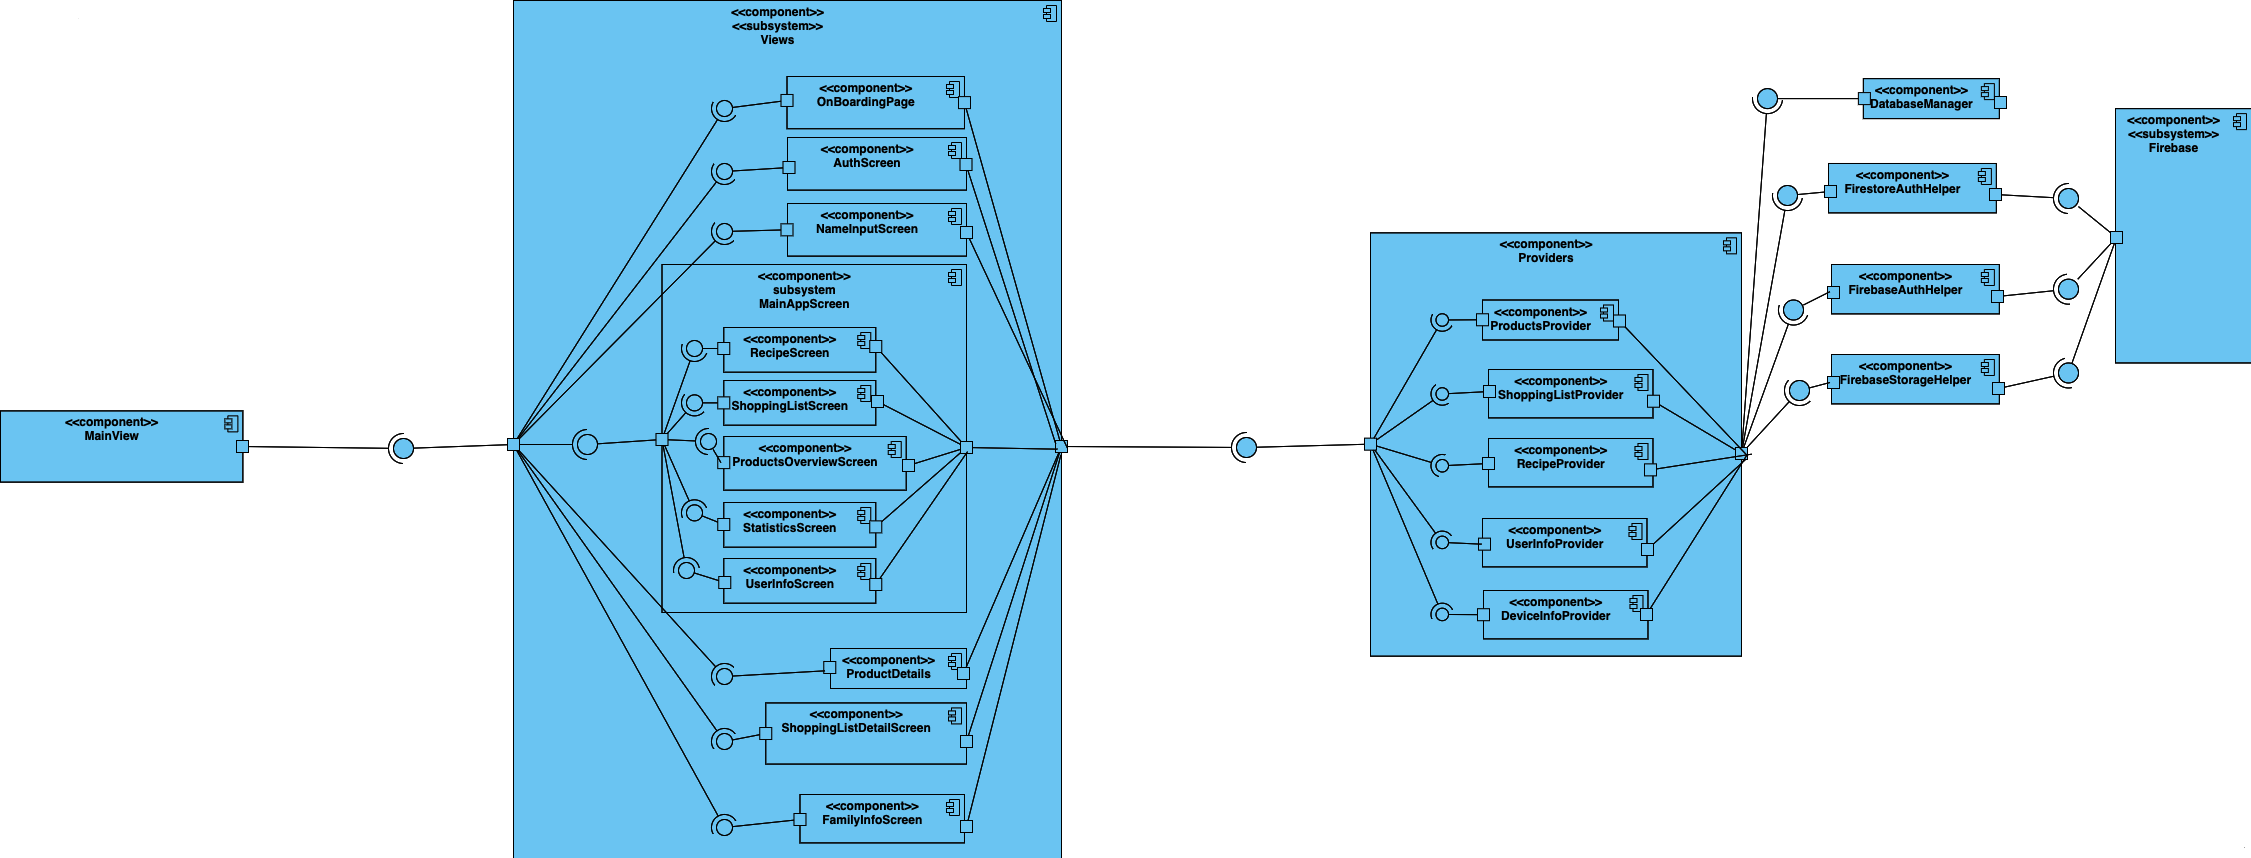
\includegraphics[scale = 0.37]{./Images/component.png}}
\vspace*{-1cm}
    \caption{Component diagram}
    \vspace*{-12cm}
\end{figure}
\fillandplacepagenumber
\end{landscape}


\subsection{Mobile Application}
The application server must handle the business logic, the connections with the
data layer, and also have to manage the different ways of accessing the services
from different clients. To comply with all these requirements, it must provide
interfaces to connect with all the previously mentioned components.
In particular the application rely on Google's Firebase.
Firebase is a Backend-as-a-Service (Baas). It provides a variety of tools and services. It is built on Google’s infrastructure.
Firebase is categorized as a NoSQL database program, which stores data in JSON-like documents.

\subsection{Application server}
The implementation of the mobile application must be autonomous from the structure of the application server. The UI must respect the design guidelines provided by Google's Material Design.
As stated before, application is developed using Flutter, which is a framework base on the Dart programming language.

To separate application states and UI, an external package called \textbf{Provider} is used.
It does mainly two jobs:
\begin{itemize}
    \item Separates state from UI
    \item Manages rebuilding UI based on state changes
\end{itemize}
Which makes loads of things simpler, from reasoning about state, to testing to refactoring. It makes codebase scalable.
It can be considered a low boiler-plate way to separate business logic from  widgets in apps.
In addition to using Providers, other external packages have been used(non-exhaustive list):
\begin{itemize}
    \item \textbf{sqflite: }SQLite plugin for Flutter
    
    \item \textbf{http: }contains a set of high-level functions and classes that make it easy to consume HTTP resources
    
    \item \textbf{flutter scandit: }barcode and qrcode scanner
    
    \item \textbf{shared preferences: }Wraps platform-specific persistent storage for simple data 
    
    \item \textbf{syncfusion flutter charts: }data visualization library charts
    
    \item \textbf{firebase: }
    \begin{itemize}
        \item \textbf{cloud firestore: }cloud-hosted, NoSQL database accessible directly via native SDKs
        \item \textbf{firebase storage: }is a service used to store and download files generated directly by clients
        \item \textbf{firebase auth: }firebase authentication API
    \end{itemize}
    
    \item \textbf{google sign in: }API to manage Google login and registration
    \item \textbf{flutter facebook auth: }API to manage Facebook login and registration
    \item \textbf{openfoodfacts: }package for the Open Food Facts API
    
    \item \textbf{testing: }
    \begin{itemize}
        \item \textbf{mockito: }testing framework
        \item \textbf{firebase auth mocks: }unit tests involving Firebase Authentication
        \item \textbf{build runner: }provides general-purpose commands for generating files, and for optionally testing the generated files or serving both source and generated files
        \item \textbf{fake cloud firestore: }Fakes to write unit tests for Cloud Firestore
        \item \textbf{google sign in mocks: }mocks for google sign in package, used for testing purposes
    \end{itemize}
    
\end{itemize}

Furthermore to get data about \texit{products} and \textit{recipes}, also external services are used.
\textbf{OpenFoodFacts }is used for retrieving information about a product given a barcode.
\textbf{Spoonacular API} is used for retrieving recipes and detail about a recipe.

\subsection{Database and Storage}
\section{Deployment view}
This section shows the physical distribution of the system, that is, the environment in which the system runs. Specifically, Figure xxx, shows the structure of the hardware component that execute the software.

\begin{figure}[H]
  \hspace*{-2cm}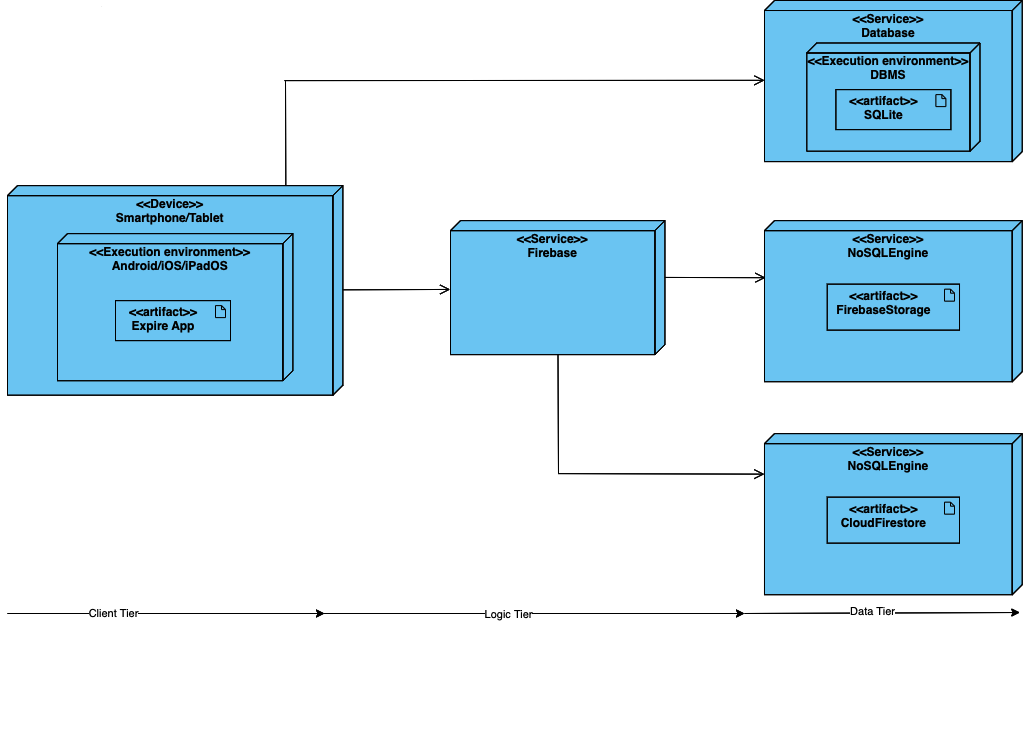
\includegraphics[scale=0.45]{./Images/Deployment.png}
  \caption{Deployment diagram}
\end{figure}
\section{Runtime view}
\section{Selected architectural styles and patterns}
\section{Other design decisions}


\subsection{Security}

\chapter{User interface design}


\chapter{Implementation and Testing strategy}
Testing is one of the most important parts of a software development.
This phase allows to go through all the possible cases that can take place when the project goes live.
Over 75 tests have been done, only the main components have been tested.
Several external libraries are also used:
\begin{itemize}
    \item \textit{mockito}
    \item \textit{firebase\textunderscore auth\textunderscore mocks}
    \item \textit{build\textunderscore runner}
    \item \textit{fake\textunderscore cloud\textunderscore firestore}
    \item \textit{google\textunderscore sign\textunderscore in\textunderscore mocks}
    \item \textit{firebase\textunderscore storage\textunderscore mocks}
\end{itemize}






\section{Unit testing}
We used a typical stub-driver approach to test the functionalities of main components of our applications. 
\newline
\newline
\hspace*{-1cm}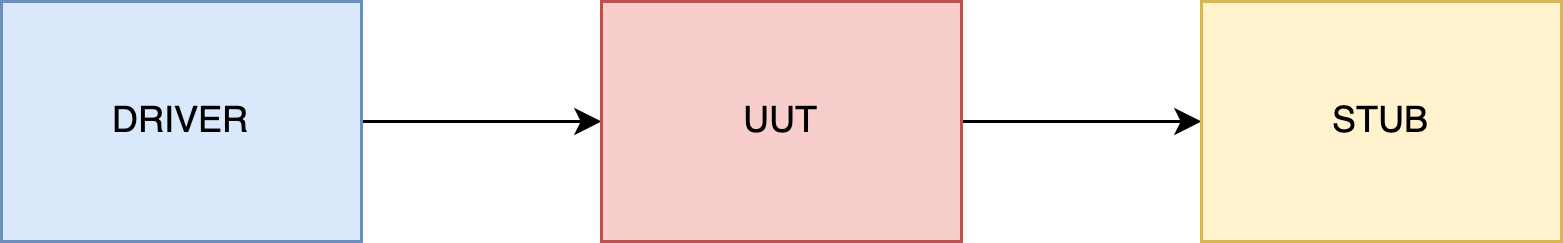
\includegraphics[width=14cm,keepaspectratio]{Images/testing/stub_driver.png}
\newpage
\noindent The tested components have been
\begin{itemize}
    \item[--] FirebaseAuthHelper
    \item[--] FirestoreHelper
    \item[--] ProductsProvider
    \item[--] ShoppingListProvider
\end{itemize}

\begin{wrapfigure}{r}{0.35\textwidth}
  \begin{center}
    \vspace*{-1cm}
\includegraphics[width=0.4\textwidth]{Images/testing/logo.png}
  \end{center}
\end{wrapfigure}
To mock their dependencies and create stubs, we used \textit{Mockito}, a powerful library that helps generating stubs.
In order for those components to be testable, we had to perform a refactoring to make them compliant to testable standard structure. One of the most important thing was to be able to inject dependencies via the constructor to create stubs for internal dependencies. We managed to accomplish this by dynamically resolve ad runtime the possibility to instantiate the object with some or all its dependencies mocked.
\newline
\newline
\begin{center}
    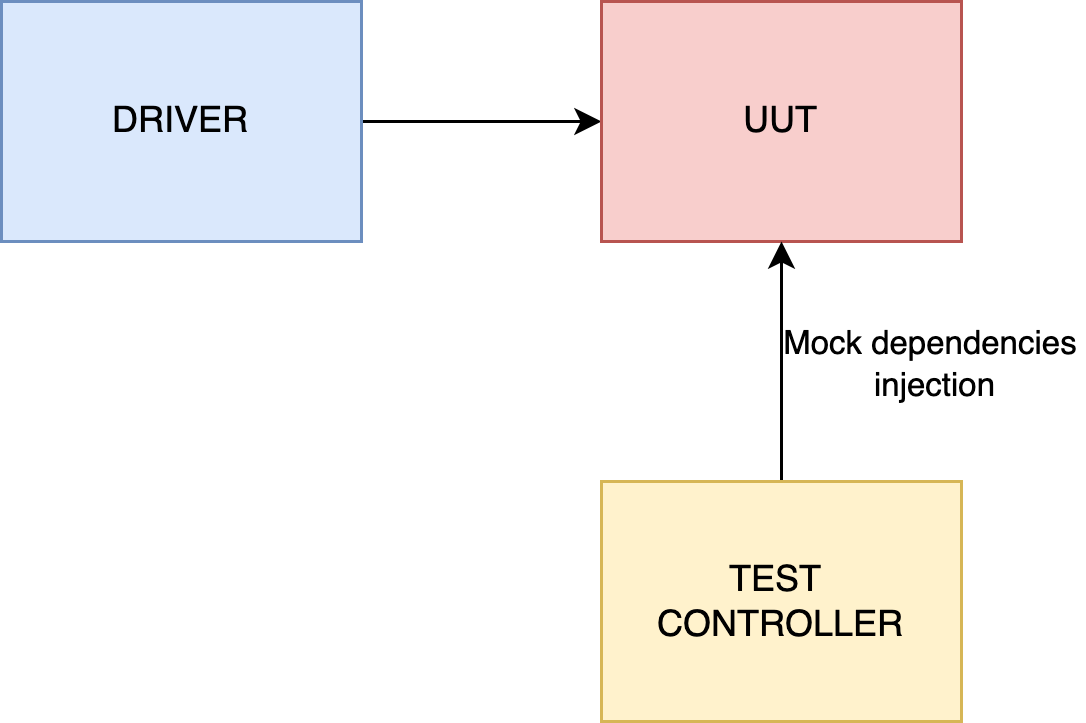
\includegraphics[width=8cm,keepaspectratio]{Images/testing/stub_driver_injection.png}
\end{center}

\noindent All of those components have been heavily tested in all of their use cases. We manage to obtain 60 tests (number also given from their complexity and dimension).
\newline
\newline
\noindent To perform assertions and evaluate tests we used the implemented flutter library called \textit{flutter\_test.dart}.

\newpage
\section{Widget testing}
Widget testing aims to test UI behavior to certain actions and it's not about functionalities and logic like the unit testing.
This type of testing is made available thanks to a \textit{Widget tester} library embedded in the flutter SDK.
\newline
\newline
\noindent The main widget tested were the sign up, sign in and the add modal product.
\newline
\newline
\noindent There it presents once again the need of using stubs because of internal dependencies inside screens and widget. The difference with the unit testing is the impossibility to perform a large scale refactoring since implementing an injectable constructor would be a tedious and very long task. We solved this by using a \textit{dependencies provider} that is responsible for providing dependencies to each widget requiring it. By doing this, each widget has dependencies fetching completely transparent while we can inject the dependencies provider with mocks to be served to widgets.

\begin{center}
    \vspace{1cm}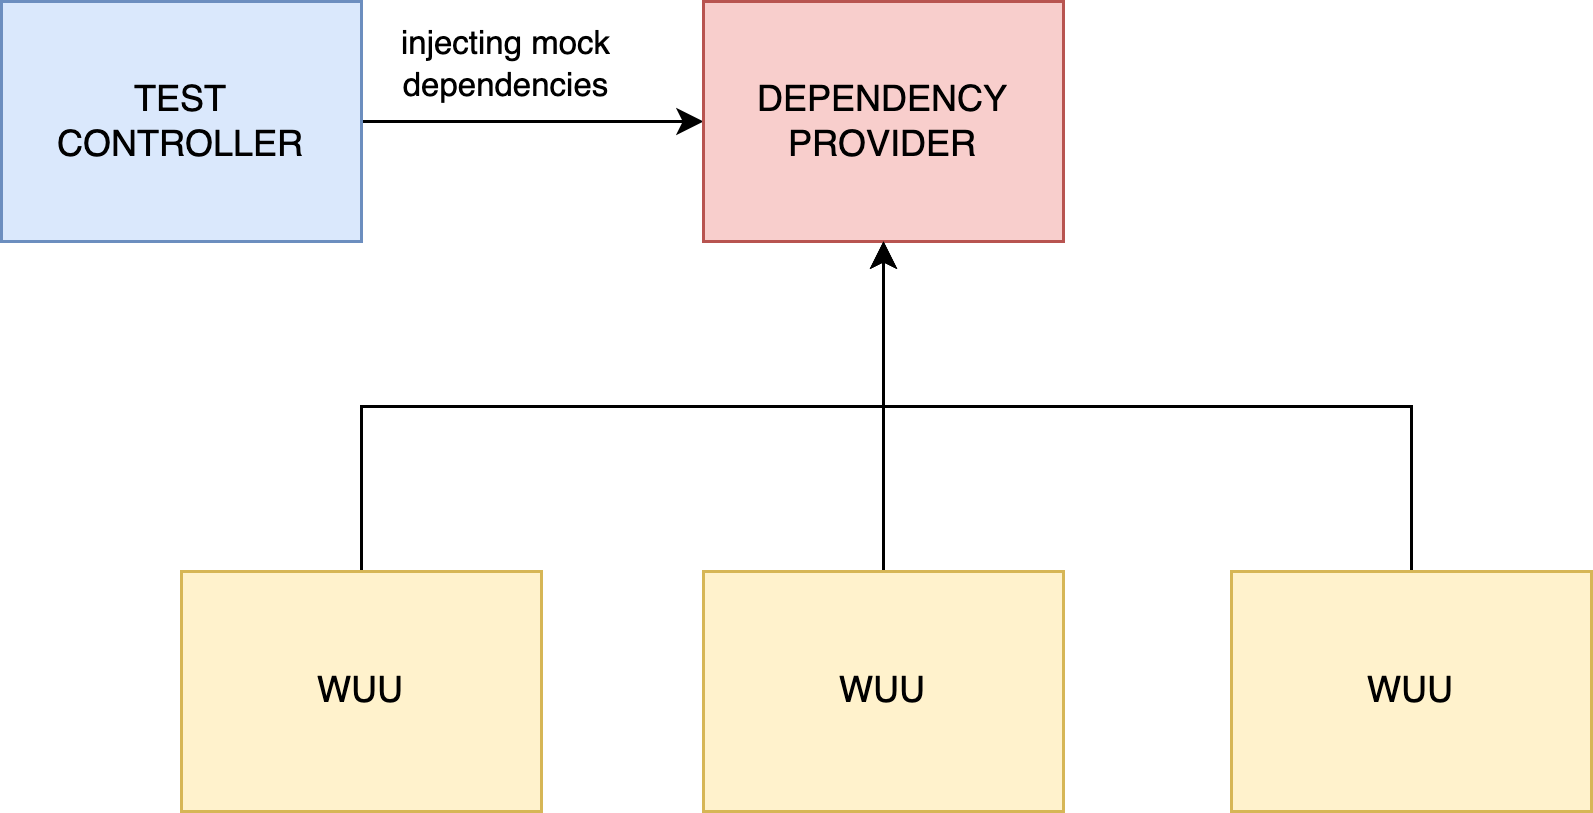
\includegraphics[width=12cm,keepaspectratio]{Images/testing/widget_testing.png}
\end{center}


\newpage
\section{Monkey testing}
Monkey testing is a technique where the user tests the application by providing random inputs and checking behaviour, or seeing whether the application or system will crash.
This test has been done using \textit{Firebase Test Lab}, that is an application-testing infrastructure offered by Google Firebase.
It permits to define different device configurations' collection on which application can be tested. Every device configuration collection works on a specific range of device types, language, and orientation configuration options.
Every test is performed via virtual and physical devices located at the Google data center.
When a test is run against devices and configurations selected, \textit{Test Lab} runs the test and display the results as a \textbf{text matrix}.
\newline
\textbf{Devices x Test Executions = Test Matrix}
\begin{figure}[H]
   \centering
  \centerline{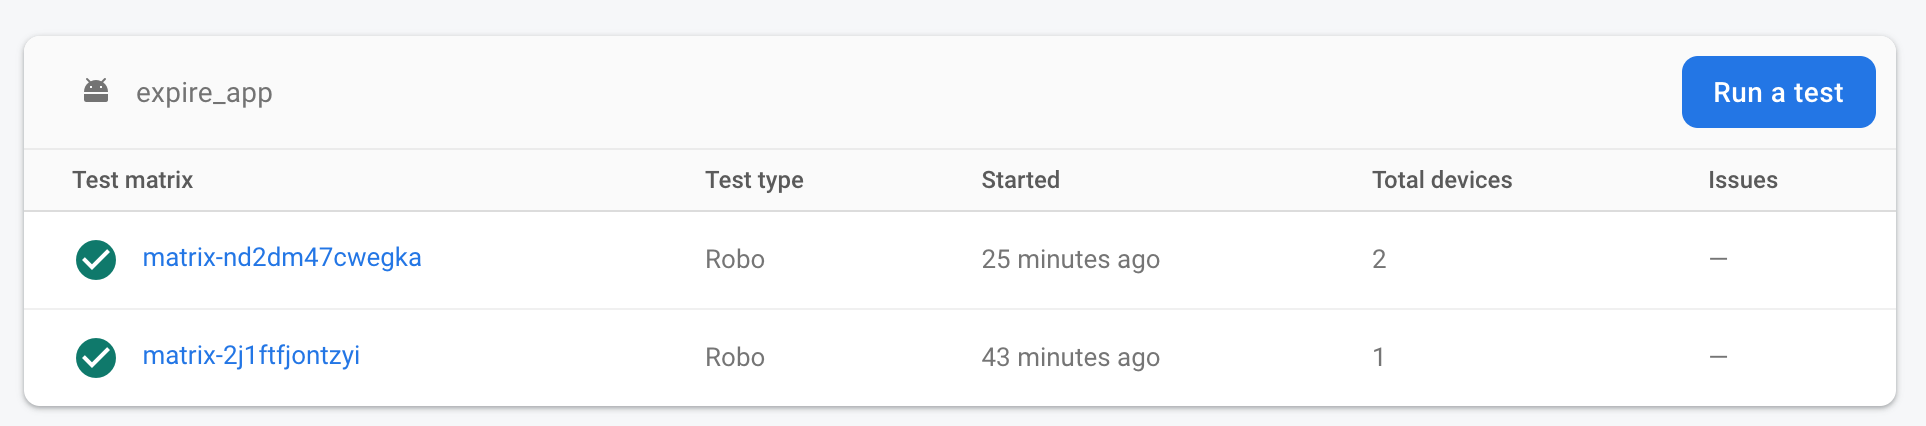
\includegraphics[width=150mm,scale=0.9]{./Images/testing/testing1.png}}
  \caption{Matrix test}
\end{figure}

Another test performed with \texit{Test Lab} is so called \textbf{robo test}.
It analyzes the structure of app's UI and explores it methodically, automatically simulating user activities.
This test captures log files, saves a series of annotated screenshots, and then creates a video form those screenshots to show the simulated operations that it performed.
\begin{figure}[H]
   \centering
  \centerline{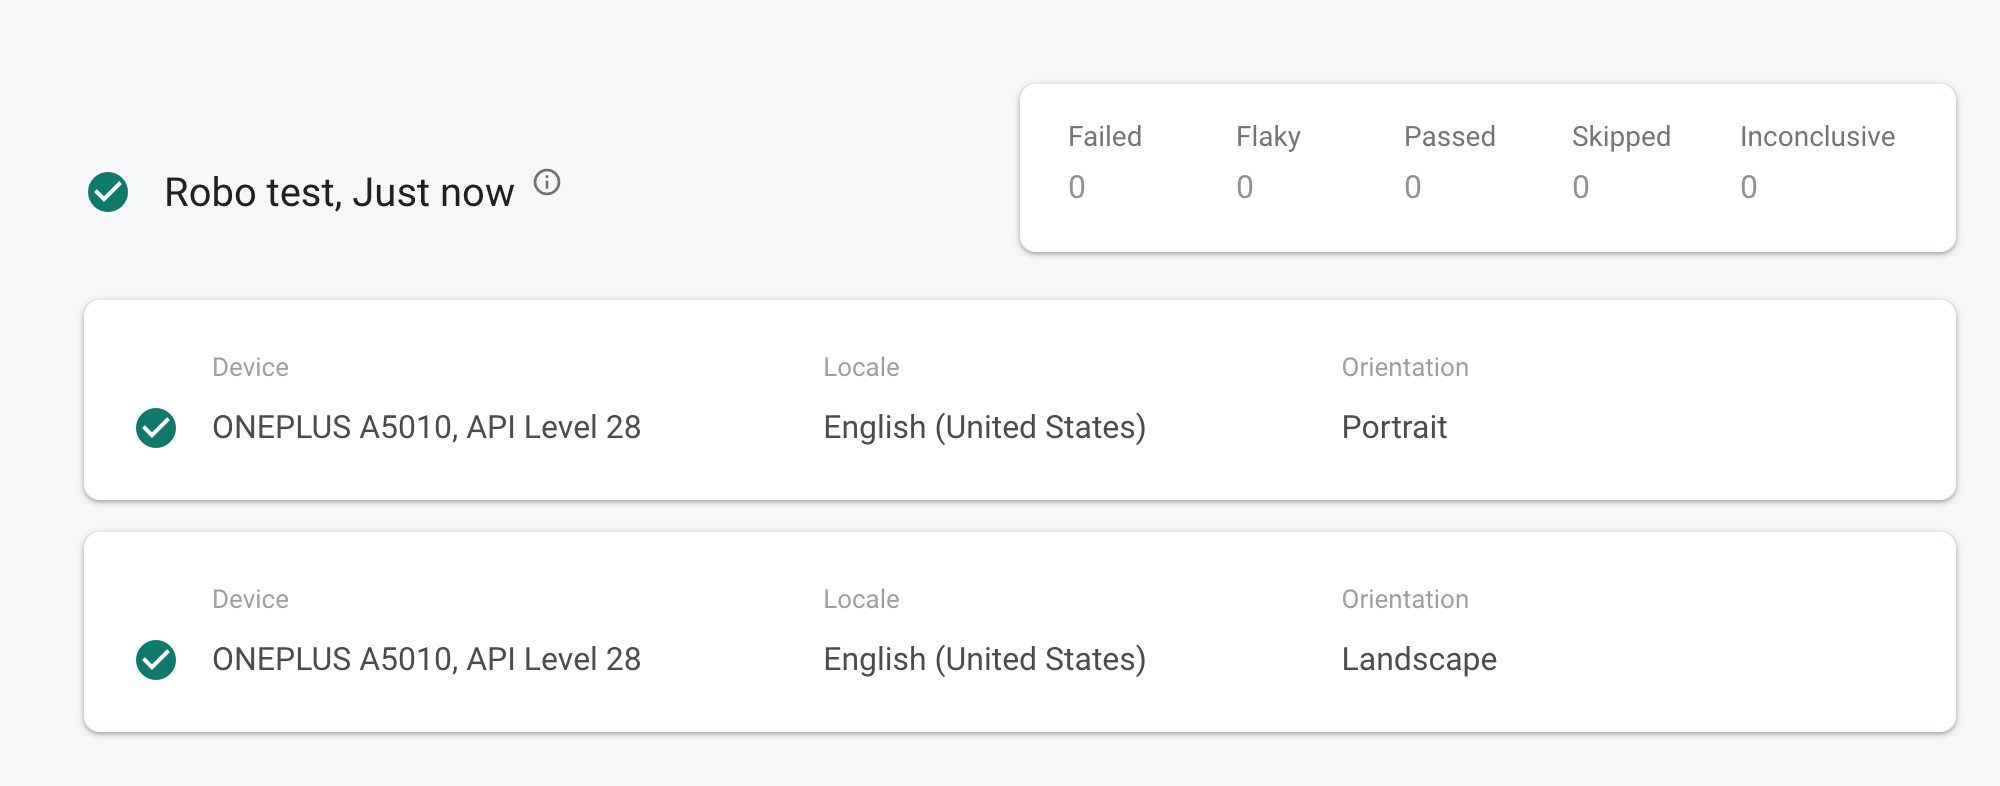
\includegraphics[width=150mm,scale=0.9]{./Images/testing/testing2.png}}
  \caption{Robo test}
\end{figure}
\chapter{Future development}


\section{Future Plans}
As future development, we would like to fully take advantage of cross platform development offered by Flutter framework, to do so implement also the notification system, explained in section 4.4, into iOS and iPadOS environments.
\newline
Moreover our team has in plan to exploit more the interaction with the final user, for eg. by implemeting a favourite section, where the user can view recipes added to favourite



\end{document}
